% Иллюстрация к def:ValiantSubmatrix: подматрица с вершиной (a,b) и размером s
% и влияющее множество I_m. n=12, a=5, b=7, s=3 (a+b=n => подматрица центрирована).
% Координаты: P(i,j) = ((i+j)/2, (j-i)/2); основание треугольника -- диагональ i+1=j.
% I_m -- буквально по def:ValiantInfluencing (асимметрично): левая часть охватывает
% s строк i (a-s<i<=a), правая -- лишь s-1 столбец j (b<j<b+s), поэтому левая шире.
% Цвета -- полупрозрачные заливки оригинального изображения, скомпозитированные
% на белый фон.
\definecolor{SubmatrixBlue}{HTML}{c7d7f0}
\definecolor{SubmatrixPurple}{HTML}{a78c96}

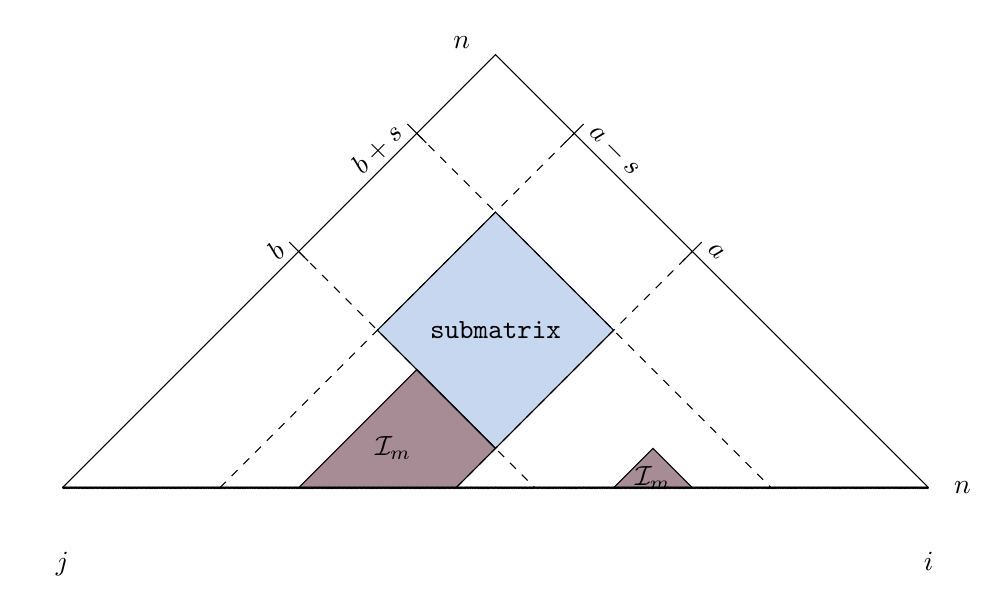
\begin{tikzpicture}
  % Треугольник таблицы: BL=P(0,1), TOP=P(0,n), BR=P(n-1,n)
  \coordinate (BL)  at (0.5,0.5);
  \coordinate (TOP) at (6,6);
  \coordinate (BR)  at (11.5,0.5);

  % Квадрат подматрицы: левый P(a-s,b), нижний P(a,b), правый P(a,b+s), верхний P(a-s,b+s)
  \coordinate (dmL) at (4.5,2.5);
  \coordinate (dmB) at (6,1);
  \coordinate (dmR) at (7.5,2.5);
  \coordinate (dmT) at (6,4);

  % I_m по определению (асимметрично):
  % левая часть {a-s<i<=a, j<=b} -- четырёхугольник P(3,4),P(3,7),P(5,7),P(5,6)
  \coordinate (imL1) at (3.5,0.5);
  \coordinate (imL2) at (5,2);
  \coordinate (imL3) at (6,1);
  \coordinate (imL4) at (5.5,0.5);
  % правая часть {b<=i<j, j<b+s} -- треугольник P(7,8),P(7,9),P(8,9)
  \coordinate (imR1) at (7.5,0.5);
  \coordinate (imR2) at (8,1);
  \coordinate (imR3) at (8.5,0.5);

  % Концы пунктирных линий (продолжения сторон квадрата до границ таблицы)
  \coordinate (jb0)  at (3.5,3.5); % j=b на левом крае
  \coordinate (jb1)  at (6.5,0.5); % j=b на основании
  \coordinate (jbs0) at (5,5);     % j=b+s на левом крае
  \coordinate (jbs1) at (9.5,0.5); % j=b+s на основании
  \coordinate (ia0)  at (5.5,0.5); % i=a на основании
  \coordinate (ia1)  at (8.5,3.5); % i=a на правом крае
  \coordinate (ias0) at (2.5,0.5); % i=a-s на основании
  \coordinate (ias1) at (7,5);     % i=a-s на правом крае

  % Закраски
  \fill[SubmatrixPurple] (imL1) -- (imL2) -- (imL3) -- (imL4) -- cycle;
  \fill[SubmatrixPurple] (imR1) -- (imR2) -- (imR3) -- cycle;
  \fill[SubmatrixBlue] (dmL) -- (dmB) -- (dmR) -- (dmT) -- cycle;

  % Пунктирные линии
  \draw[dashed] (jb0)  -- (jb1);
  \draw[dashed] (jbs0) -- (jbs1);
  \draw[dashed] (ia0)  -- (ia1);
  \draw[dashed] (ias0) -- (ias1);

  % Контур: боковые стороны и зигзаг на основании
  \draw (BL) -- (TOP) -- (BR);
  \draw[decorate, decoration={zigzag, amplitude=0.12, segment length=0.3}] (BL) -- (BR);

  % Контур квадрата и областей I_m
  \draw (dmL) -- (dmB) -- (dmR) -- (dmT) -- cycle;
  \draw (imL1) -- (imL2) -- (imL3) -- (imL4) -- cycle;
  \draw (imR1) -- (imR2) -- (imR3) -- cycle;

  % Тики на краях
  \draw (3.38,3.62) -- (3.62,3.38);
  \draw (4.88,5.12) -- (5.12,4.88);
  \draw (8.38,3.38) -- (8.62,3.62);
  \draw (6.88,4.88) -- (7.12,5.12);

  % Метки на краях (повёрнуты вдоль края)
  \node[rotate=45, anchor=east]  at (3.35,3.65)  {$b$};
  \node[rotate=45, anchor=east]  at (4.85,5.15)  {$b+s$};
  \node[rotate=-45, anchor=west] at (8.65,3.65)  {$a$};
  \node[rotate=-45, anchor=west] at (7.15,5.15)  {$a-s$};

  % Метки углов и осей
  \node[anchor=east]  at (0.3,0.5)  {$\varnothing$};
  \node[anchor=west]  at (11.7,0.5) {$n$};
  \node[anchor=east]  at (5.8,6.15) {$n$};
  \node[anchor=west]  at (6.2,6.15) {$\varnothing$};
  \node[anchor=north] at (0.5,-0.2) {$j$};
  \node[anchor=north] at (11.5,-0.2) {$i$};

  % Подписи
  \node at (6,2.5) {\texttt{submatrix}};
  \node at (4.7,1.0) {$\mathcal{I}_m$};
  \node at (8,0.62) {$\mathcal{I}_m$};
\end{tikzpicture}
